\section{Class Interfaces}
The following is a description of the public functions of all public classes.
Many classes have inner private classes they use for convenience, however to
simplify interaction between parts of our system ('modules') we have very few
convenience classes.

\begin{table}[H]
    \centering
    \begin{tabular}{p{1cm}p{1cm}p{3cm}}
    return & function & description\\ \hline
    void   & main() & (static) starts the server\\
    \end{tabular}
    \caption{Server}
\end{table}

\begin{table}[H]
    \centering
    \begin{tabular}{p{1cm}p{1cm}p{9cm}}
    return & function & description\\ \hline
    void   & main()   & (static) constructs and starts all necessary classes and threads, runs the main loop\\
    \end{tabular}
    \caption{Client}
\end{table}

\begin{table}[H]
    \centering
    \begin{tabular}{p{1cm}p{2.8cm}p{9cm}}
    return   & function            & description\\ \hline
    N/A      & NetworkConnection() & Constructs a NetworkConnection and connects to the given URL (through tor)\\
    void     & run()               & periodically download new messages until asked to close, downloaded messages are stored in a FIFO buffer\\
    void     & close()             & kills the thread started by run()\\
    boolean  & hasMessage()        & return true if there is a message in the buffer, false otherwise\\
    String   & getMessage()        & return the oldest message in the buffer\\
    
    boolean  & claimName()     & claim a given username, returns true on success, false otherwise\\
    void     & revokeKeypair() & revokes your keypair\\
    void     & pdata()         & adds or updates profile information\\
    void     & chat()          & begins or continues a conversation\\
    void     & post()          & post a message to your wall\\
    void     & fpost()         & post a message to a friends wall\\
    void     & comment()       & comment on a comment or post\\
    void     & like()          & like a comment or post\\
    void     & event()         & create an event\\
    \end{tabular}
    \caption{NetworkConnection}
\end{table}

\begin{table}[H]
    \centering
    \begin{tabular}{p{1.4cm}p{3.3cm}p{9cm}}
    return     & function        & description\\ \hline
    boolean    & keysExist()     & (static) return true if the user has a keypair, false otherwise\\
    void       & keyGen()        & (static) generate a keypair for the user\\
    PublicKey  & getPublicKey()  & (static) returns the users public key\\
    PrivateKey & getPrivateKey() & (static) returns the users private key\\

    String     & sign()      & (static) returns an RSA signature of the passed string\\
    boolean    & verifySig() & (static) returns true if author signed msg, false otherwise\\
    String     & encrypt()   & (static) returns an encrypted message constructed from the passed parameters\\
    Message    & decrypt()   & (static) decrypts the passed string, returns the appropriate message, on failure a NULL message is returned\\
    String    & base64Encode() & (static) base64 encodes the passed data, returns the string\\
    byte[]    & base64Decode() & (static) base64 decodes the passed data, returns the byte[]\\
    String    & encodeKey()    & (static) encodes a public key as a string, returns that string (X509)\\
    PublicKey & decodeKey()    & (static) decodes a public key encoded as a string, returns that public key(X509)\\
    String    & hash ()        & (static) returns the SHA256 hash the the passed string as a hex string\\
    int       & rand ()        & (static) returns a pseudorandom value <= max and >= min\\
    \end{tabular}
    \caption{Crypto}
\end{table}

\begin{table}[H]
    \centering
    \begin{tabular}{p{1cm}p{2.6cm}p{9cm}}
    return & function & description\\ \hline
    void   & parse()  & (static) parses a sting message, records parsed data in the database\\
    \end{tabular}
    \caption{Parser}
\end{table}

\begin{table}[H]
    \centering
    \begin{tabular}{p{3cm}p{3cm}p{9cm}}
    return                & function       & description\\ \hline
    
    void                  & addClaim()     & adds a username CLAIM message\\
    pair<string,string>[] & getClaims()    & gets all CLAIMs to usernames\\
    string[]              & getUsernames() & gets all usernames\\
    
    void                    & addRevocation()  & adds a keypair revocation\\
    pair<PublicKey, long>[] & getRevocations() & gets all revocations\\
    boolean                 & isRevoked()      & returns the time a key was revoked, if the given key has not been revokes then 0 is returned.\\
    
    void   & addPData() & adds (or amends existing) profile data\\
    string & getPData() & gets the specified piece of profile data for a specified user\\
    
    void                  & createChat() & creates new chat\\
    pair<string,string>[] & getChat()    & returns messages from a given chat\\
    void                  & addToChat()  & adds a post to a given chat\\
    
    void                  & addPost()  & creates new post, on your or another's wall\\
    pair<string,string>[] & getPosts() & gets all posts either within timeframe, or from certain people within a timeframe\\
    
    void                  &  addComment() & adds a comment onto post or comment\\
    pair<string,string>[] & getComments() & gets all comments for a post or comment\\
    
    void     & addLike() & likes a post or comment\\
    String[] & getLikes() & gets all likes from certain person within a timeframe\\
    int      & countLikes() & gets the number of likes for a comment or post\\
    
    void                & addEvent()     & adds new event\\
    pair<string,long>[] & getEvent()     & gets all events within timeframe\\
    void                & acceptEvent()  & accepts notification of an event\\
    void                & declineEvent() & declines notification of an event\\
    
    void        & addKey()  & adds a public key to the DB\\
    PublicKey[] & getKey()  & gets the public key for a usernamne, or all which are stored)\\
    string      & getName() & gets a username for the given public key\\

    void & addCategory()   & adds a new category to the DB\\
    void & addToCategory() & adds a user to a category\\
    \end{tabular}
    \caption{Database}
\end{table}

\begin{table}[H]
    \centering
    \begin{tabular}{p{1cm}p{2.6cm}p{9cm}}
    return  & function    & description\\ \hline
    N/A     & GUI()       & Constructs a GUI\\
    void    & run()       & continually updates the GUI from the DB\\
    void    & close()     & kills the GUIServer thread\\
    boolean & isRunning() & returns true if the GUIServer is running, false otherwise\\
    \end{tabular}
    \caption{GUI}
\end{table}

\begin{table}[H]
    \centering
    \begin{tabular}{p{1cm}p{2.6cm}p{9cm}}
    return  & function       & description\\ \hline
    N/A     & Message()      & Constructs a message with given data\\
    
    Message & parse()        & (static) parses the string representation of a message into a message\\
    
    String  & toString()     & creates a string representation of the message\\
    String  & getCmd()       & returns the type of message\\
    String  & getContent()   & returns the content of the message\\
    String  & getSig()       & returns the RSA signature on the message\\
    long    & getTimestamp() & returns the timestamp on the message\\
    \end{tabular}
    \caption{Message}
\end{table}

\begin{table}[H]
    \centering
    \begin{tabular}{p{1cm}p{2cm}p{9cm}}
    return & function & description\\ \hline
    
    N/A    & Pair()   & Constructs a pair with given data\\
    A      & first()  & returns the first value passed to the constructor\\
    B      & second() & returns the second value passed to the constructor\\
    \end{tabular}
    \caption{Pair\textless A, B\textgreater }
\end{table}

%\clearpage
\section{Class Diagram}
\begin{figure}[H]
    \centering
    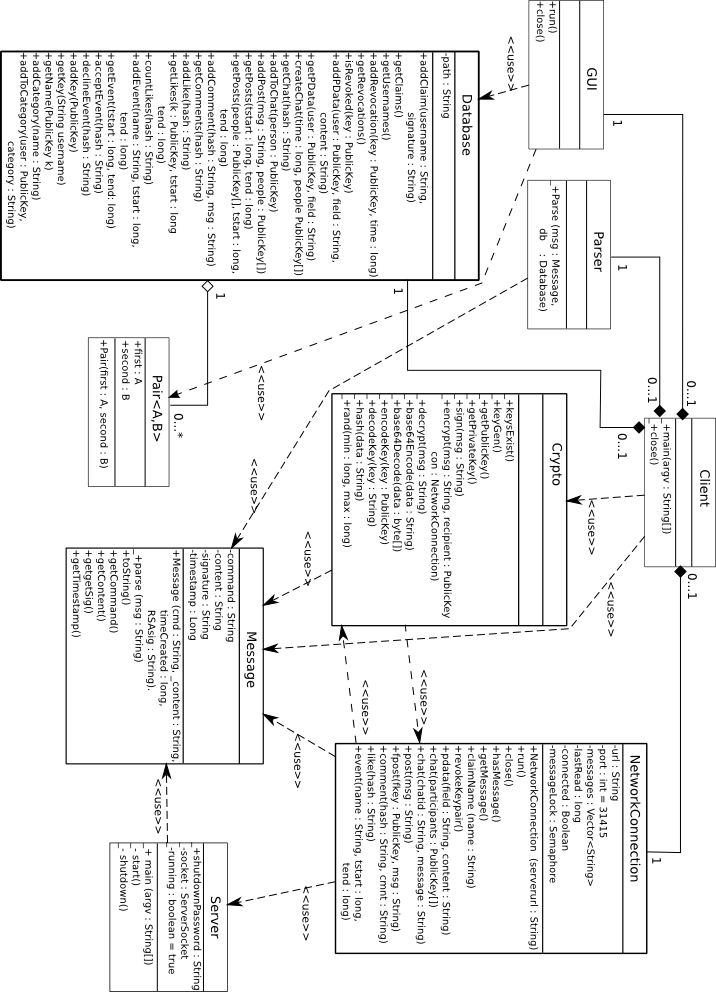
\includegraphics[width=\textwidth]{images/design/class_diagram.png}
    \caption{UML Class Diagram}
    \label{fig:class_diagram}
\end{figure}
